\section{Einleitung}
Ein großer Teil der Forschung in der Physik umfasst das Schreiben und Entwickeln umfangreicher Programmcodes. Diese werden meist über Jahre oder gar Jahrzehnte hinweg aufgebaut. Viele Codes werden von großen Gruppen gemeinsam weiter entwickelt. Um Programmcode effizient zu dokumentieren und Änderungen auch Jahre später noch rückverfolgbar zu machen wurden Versionskontrollsysteme genutzt. Diese Systeme sollen einen Überblick über den Verlauf von Änderungen verschaffen, aber auch die Zuordnung von Änderungen zu Personen ermöglichen. Mittlerweile nutzen viele Entwickler Git als Versionskontrolle. Dafür werden zumeist auch öffentliche Server (\url{Gitlab.com} oder \url{Github.com}) genutzt um den Code der Community zur Verfügung zu stellen\footnote{Auch der Quelltext dieser Arbeit steht auf Github zur Verfügung unter: {\url{https://github.com/tillhanke/Git-Einfuehrung}}}. 

Eine Bereitstellung von Quellcode sollte in wissenschaftlichen Arbeiten standardisiert werden, und Git bietet genau solch einen Standard.

In dieser Arbeit sollen Grundlagen der Arbeit mit Git erklärt werden. Der Fokus liegt dabei auf dem Arbeiten alleine mit einer dezentralen Sicherung des Codes.

Alle Instruktionen in dieser Arbeit beziehen sich auf Linux Betriebssysteme. Die meisten der angegebenen Befehle werden auch auf MacOS Systemen funktionieren. Git ist auch für Windows OS verfügbar jedoch wird darauf in dieser Arbeit nicht eingegangen. Auch die Installation von Git auf den genutzten Maschinen wird vorausgesetzt.

Diese Arbeit orientiert sich maßgeblich an dem Kostenlos verfügbaren Buch \cite{ProGit}, in dem Git sehr ausführlich erklärt wird. Für den interessierten Leser sind dort umfangreiche Erklärungen zu fortgeschrittenen Methoden.

\subsection{Versionskontrolle}
Das Ziel einer Versionskontrolle wie Git ist es die Änderungen an einem Projekt zu dokumentieren. In Abb. \ref{fig:vers-kontrol}
ist eine solche Protokollierung visualisiert. Um Änderungen zu dokumentieren werden zu jeder Änderungen Kommentare hinzugefügt - sogenannte \qq{Commit-Messages}. Diese sollen das spätere zurückverfolgen der Änderungen vereinfachen. Um Speicherplatz zu sparen werden in der Versionskontrolle möglichst nicht alle Dateien zu jedem Zeitpunkt gespeichert. Es wird nur einmal (zum Zeitpunkt der Erstellung) die komplette Datei gesichert. Danach werden von jeder Datei nur Informationen über die Änderungen abgespeichert.
\begin{figure}[!h]
    \centering
    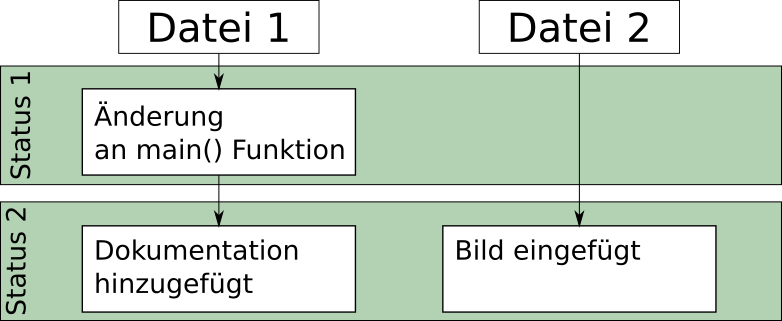
\includegraphics[width=0.9\textwidth]{Bilder/Versioncontrol.png}
    \caption{Beispiel einer Versionskontrolle von drei Änderungen an zwei Dateien desselben Projekts. Eingezeichnet sind zwei protokollierte Stadien des Projekts. Zu jeder Änderung ist ein Änderungskommentar angegeben.}
    \label{fig:vers-kontrol}
\end{figure}